\documentclass[dvipdfmx,twoside]{jsarticle}
\usepackage{amsmath,amssymb}
\usepackage{CJKutf8}
\usepackage{okumacro}
\usepackage{booktabs}
\usepackage{array}
\usepackage{xcolor}
\usepackage{colortbl}
\usepackage{tipa}
\usepackage{tikz}
\usepackage{fancybox}
\usepackage{wasysym}
\usepackage{pifont}
\usepackage{graphicx}
\usepackage{wrapfig}
\usepackage{geometry}
\geometry{margin=2cm}
\usepackage{fancyhdr}
\usepackage{pgfplots}
\pgfplotsset{compat=1.18}
\usepackage[utf8]{inputenc}
\usepackage{CJK}
\usetikzlibrary{positioning, intersections, calc, arrows.meta, math, through}
\usepackage{tcolorbox}
\tcbuselibrary{theorems,breakable}
\usepackage{enumerate}
\usepackage{titlesec}

% 自定义subsubsection格式
\titleformat{\subsubsection}
  {\normalfont\normalsize\bfseries}
  {1.\arabic{subsubsection}}
  {1em}
  {}
% 设置页面样式
% \pagestyle{fancy}
% \fancyhf{}
% \renewcommand{\headrulewidth}{0pt}
% \fancyhead[RO]{数学–\thepage}
% \fancyhead[LE]{数学–\thepage}

% 重新定义 plain 样式
% \fancypagestyle{plain}{%
%   \fancyhf{}%
%   \renewcommand{\headrulewidth}{0pt}%
%   \fancyhead[RO]{数学-\thepage}%
%   \fancyhead[LE]{数学-\thepage}%
% }
\newtcbtheorem[]{reidai}{例題}
{fonttitle=\gtfamily\sffamily\bfseries\upshape\large,
colframe=black,colback=black!15!white,
rightrule=1pt,leftrule=1pt,bottomrule=2pt,
colbacktitle=black,theorem style=standard,breakable,arc=10pt}
{tha}
\newcommand{\kai}%解答
{\noindent
\begin{tikzpicture}[scale=0.2, baseline=2.8pt]
\draw (3.3,1) node{\large\textgt{解 答}};
\draw[thick, rounded corners=3pt,] (0,0)--(6.5,0)--(6.5,2.2)--(0,2.2)--cycle;
\end{tikzpicture}\;}
\newcommand{\shomei}%証明
{\noindent
\begin{tikzpicture}[scale=0.2, baseline=2.8pt]
\draw (3.3,1) node{\textgt{証 明}};
\draw[double,thick,rounded corners=3pt,] (0,0)--(6.5,0)--(6.5,2.2)--(0,2.2)--cycle;
\end{tikzpicture}\;}
%補足
\newcommand{\hosoku}{\noindent
\begin{tikzpicture}[scale=0.2, baseline=2.8pt]
\draw (6,1) node{\large\textgt{補足}};
\fill (0,1)--(1,0)--(2,1)--(1,2)--cycle;
\fill[gray] (1,1)--(2,0)--(3,1)--(2,2)--cycle;
\fill (2,1)--(3,0)--(4,1)--(3,2)--cycle;
\fill (10,1)--(11,0)--(12,1)--(11,2)--cycle;
\fill[gray] (9,1)--(10,0)--(11,1)--(10,2)--cycle;
\fill (8,1)--(9,0)--(10,1)--(9,2)--cycle;
\end{tikzpicture}\;}
%注意
\newcommand{\chui}{\noindent
\begin{tikzpicture}[scale=0.2, baseline=2.8pt]
\fill (0,0)--(6.5,0)--(6.5,2.2)--(0,2.2);
\draw (3.3,1) node[white]{\large\textgt{注意!}};
\draw[thick] (0,0)--(6.5,0)--(6.5,2.2)--(0,2.2)--cycle;
\end{tikzpicture}\;}
% 自定义A方框命令
\newcommand{\abb}[1]{%
\begin{tikzpicture}[baseline]
\node[draw=black, 
      rectangle, 
      minimum width=0.8cm, 
      minimum height=0.3cm, 
      fill=gray!25, 
      font=\bfseries,
      line width=1pt,
      inner sep=2pt,
      anchor=base] {#1};
\end{tikzpicture}%
}
\newcommand{\ab}[1]{%
\begin{tikzpicture}[baseline]
\node[draw=black, 
      rectangle, 
      minimum width=0.8cm, 
      minimum height=0.3cm, 
      font=\bfseries,
      line width=1pt,
      inner sep=2pt,
      anchor=base] {#1};
\end{tikzpicture}%
}

\newcommand{\maru}[1]{\tikz[baseline=-0.7ex]{
    \node[shape=circle,draw,inner sep=1pt,minimum size=5pt,anchor=center] {\footnotesize #1};}}
\definecolor{headercolor}{RGB}{220,220,220}
\definecolor{rowcolor1}{RGB}{245,245,245}
\definecolor{rowcolor2}{RGB}{255,255,255}

% \title{\vspace{-1.5cm} 2025年8月羚課文科数学月考 }
% \author{\textnosfal{Linc\ -\ 伊}}
\date{}
\begin{document}
\thispagestyle{empty}
\begin{CJK}{UTF8}{ipxm}  % 使用ipxm字体
  %月考表纸部分
\begin{center}

\vspace*{5cm}

% 学校logo

\includegraphics[width=5cm]{pics/1.jpg}

\vspace{2cm}

% 主标题
{\fontsize{24}{30}\selectfont\bfseries\sffamily
2025年8月\\
\vspace{1em}
羚課文科数学月考\\
\vspace{1em}
解答
}

\end{center}
%問題1の内容
\newpage
\section*{問題\textrm{I}}
\setcounter{page}{1}
\noindent
\textbf{問1}\qquad $ x^2+y^2=4 $のとき、 $ 2x+y $の最大値は$\ab{\textsf{A}}\sqrt{\ab{\textsf{B}}}$\\

2次関数$y = x^2 + 6x + 5$ のグラフを原点$(0,0)$に関して対称移動してできるグラフの方程式は\\
$$ y= \ab{\textsf{C}}\ x^2+\ab{\textsf{D}}\ x-\ab{\textsf{E}}$$
\\
\\

\kai\\

\noindent
(1)\quad $ x^2+y^2=4 $によって、 これは円の中心が$ (0,0) $、半径rが2の円である。 $ 2x+y $の最大値を $ k $とすると、 $ 2x+y=k\implies y=-2x+k\implies 2x+y-k=0$\ 
ここで、円の上に$2x+y$の最大値を得られる点$(x_0,y_0)$が存在する。よって、直線 $ 2x+y-k=0 $は円との関係は接する場合と交わる場合の2ケースだけである。したがって、
点と直線の距離の公式によって、円の中心座標を$2x+y-k=0$に代入すると $ d=\dfrac{|2\times 0+0-k|}{\sqrt{2^2+1^2}}\leq 2=r\ \implies |-k|\leq 2\sqrt{5}$となる。
$ |-k| = |k|$により、 $ |k|\leq 2\sqrt{5}\ \implies -2\sqrt{5}\leq k\leq 2\sqrt{5} $。以上より、 $ 2x+y $の最大値は $ 2\sqrt{5} $である。
\\

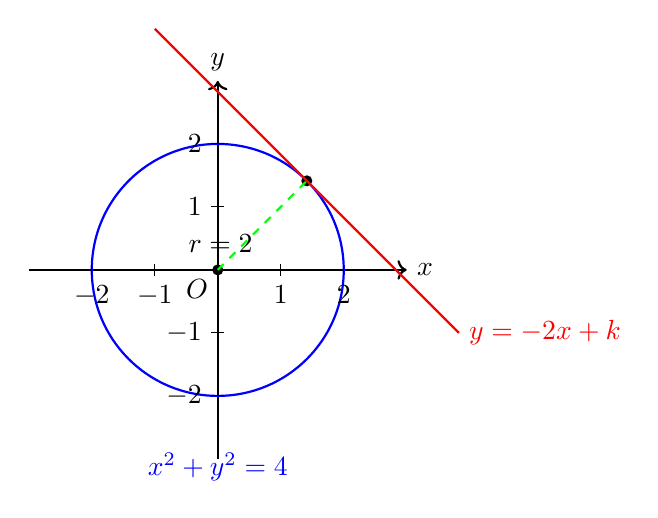
\begin{tikzpicture}[scale=0.8]
% 坐标轴
\draw[->, thick] (-3,0) -- (3,0) node[right] {$x$};
\draw[->, thick] (0,-3) -- (0,3) node[above] {$y$};

% 圆形 x^2 + y^2 = 4 (半径为2)
\draw[thick, blue] (0,0) circle (2);

% 坐标轴刻度
\foreach \i in {-2,-1,1,2} {
  \draw (\i,0.1) -- (\i,-0.1) node[below] {$\i$};
  \draw (0.1,\i) -- (-0.1,\i) node[left] {$\i$};
}

% 原点
\node[below left] at (0,0) {$O$};
\fill (0,0) circle (2.5pt);
\fill (1.414,1.414) circle (2.5pt);

% 相切直线 y = -x + 2√2 (斜率为-1)
\draw[thick, red] (-1,3.828) -- (3.828,-1) node[right] {$y = -2x + k$};

% 从圆心到直线的垂直距离
\draw[dashed, green, thick] (0,0) -- ({sqrt(2)},{sqrt(2)});

% 距离标注
\node[below left] at ({sqrt(2)/2},{sqrt(2)/2}) {$r=2$};

% 标题
\node[above] at (0,-3.5) {\color{blue}{$x^2 + y^2 = 4$}};
\end{tikzpicture}
\\

\noindent
(2)\quad 原点に関して対称移動: $x$を$-x$に、$y$を$-y$に変える。したがって、$ y=-f(-x)\implies y=-x^2+6x-5 $\\
すなわち\textcolor{red}{$y=-x^2+6x-5$}\\
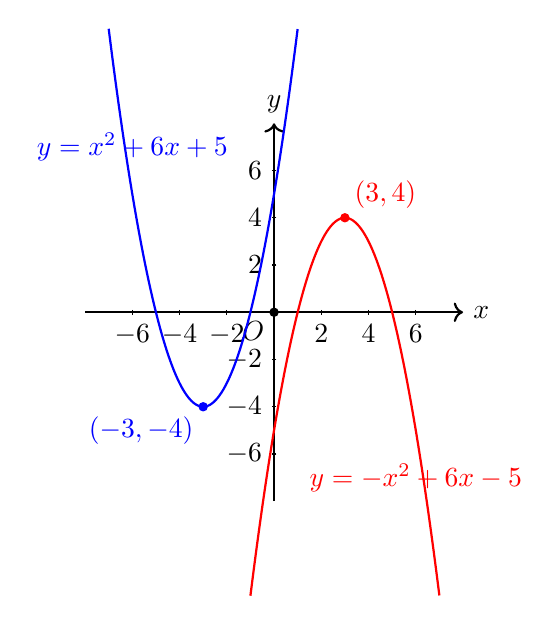
\begin{tikzpicture}[scale=0.3]
% 坐标轴
\draw[->, thick] (-8,0) -- (8,0) node[right] {$x$};
\draw[->, thick] (0,-8) -- (0,8) node[above] {$y$};

% 坐标轴刻度
\foreach \i in {-6,-4,-2,2,4,6} {
    \draw (\i,0.1) -- (\i,-0.1) node[below] {$\i$};
    \draw (0.1,\i) -- (-0.1,\i) node[left] {$\i$};
}

% 原点
\node[below left] at (0,0) {$O$};
\fill[black] (0,0) circle (0.2);

% 原函数 y = x^2 + 6x + 5
\draw[thick, blue, domain=-7:1, samples=100] 
    plot (\x, {\x*\x + 6*\x + 5});

% 对称移动后的函数 y = -x^2 - 6x - 5
\draw[thick, red, domain=-1:7, samples=100] 
    plot (\x, {-\x*\x + 6*\x - 5});

% 顶点
\fill[blue] (-3,-4) circle (0.2) node[below left] {$(-3,-4)$};
\fill[red] (3,4) circle (0.2) node[above right] {$(3,4)$};


% 函数标签
\node[blue, above] at (-6,6) {$y = x^2 + 6x + 5$};
\node[red, below] at (6,-6) {$y = -x^2 + 6x - 5$};
\end{tikzpicture}
\newpage
\noindent
\textbf{問2}\qquad $3a + 1$ が $a^2 + 6$ の約数となるような自然数 $a$ を求めよう。

\vspace{2em}

$3a + 1 = b$ とする。このとき

\vspace{1em}

\begin{center}
$a^2 + 6 = \dfrac{b^2 - \ab{\textsf{F}}\ b + \ab{\textsf{GH}}}{\ab{\textsf{I}}}$ \hspace{2em} $\cdots\cdots$ \maru{1}
\end{center}

\vspace{1em}

である。また、$b$ は $a^2 + 6$ の約数であるから、$a^2 + 6$ はある自然数 $c$ を用いて

\vspace{1em}

\begin{center}
$a^2 + 6 = bc$ \hspace{2em} $\cdots\cdots$ \maru{2}
\end{center}

\vspace{1em}
と表される。\maru{1}、\maru{2} から

\vspace{1em}

\begin{center}
$b\left(\ab{\textsf{J}}\ c - b + \ab{\textsf{K}}\right) = \ab{\textsf{LM}}$
\end{center}

\vspace{1em}

を得る。したがって、$b$ は \abb{\textsf{LM}} の約数である。この中で、$a$ が自然数となるのは $b =$ \ab{\textsf{NO}}

\vspace{1em}

である。したがって、$a = \ab{\textsf{PQ}}$ である
\\
\\

\kai\\

\noindent
(1)\quad $3a + 1 = b$とすると、$a=\dfrac{b-1}{3}$となって、$a$を$a^2+6$に代入すると、$a^2 + 6 = \dfrac{(b-1)^2}{9} + 6 = \dfrac{b^2 - 2b + 1 + 54}{9} = \dfrac{b^2 - {\color{red}{2} }b + \color{red}{55}}{\color{red}{9}}$となる。\\

\noindent
(2)\quad \maru{1}と\maru{2}の式から、 $ a^2+6=bc=\dfrac{b^2 - 2b + 55}{9}\ \implies\ 9bc-b^2+2b=55\ \implies\ b({\color{red}{9}}c-b+{\color{red}{2}})=\color{red}{55}$。\\

\noindent
(3)\quad $b$は$55$の約数である。したがって、$b$は$1,5,11,55$のいずれかである($55=55\times 1=5\times 11\times 1$)。$a$が自然数それと$b=3a+1$の条件によって、 $b\geq 4$となる。したがって、$b=5$の場合は、$a=\dfrac{b-1}{3}=\dfrac{4}{3}$であり、$a$の条件を満たさない。$b=11$の場合は、$a=\dfrac{b-1}{3}=\dfrac{10}{3}$であり、$a$の条件を満たさない。$b=55$の場合は、$ a=\dfrac{b-1}{3}=\dfrac{54}{3}=18$であり、$a$の条件を満たす。したがって、$b={\color{red}{55}},a=\color{red}{18}$が求める答えである。\\

%問題2の内容
\newpage
\section*{問題\textrm{II}}
\noindent
\textbf{問1}\qquad 異なる4つの箱がある。これらの箱に赤、黒、緑、黄の色を塗る。ただし、\\
\hspace*{1em}どの箱にも1つの色のみを使い、また同じ色の箱が2枚以上あってもよいものとする。

\vspace{1em}

(1) \hspace{1em} 全部で \ab{\textsf{ABC}} 通りの塗り方がある。

\vspace{1em}

(2) \hspace{1em} 全部の色を使う塗り方は \ab{\textsf{DE}} 通りある。

\vspace{1em}

(3) \hspace{1em} 2枚は赤で、1枚が黒、1枚が緑となるような塗り方は \ab{\textsf{FJ}} 通りある。

\vspace{1em}

(4) \hspace{1em} 3つの色を使う塗り方は \ab{\textsf{GHI}}  通りある。

\vspace{1em}

(5) \hspace{1em} 2つの色を使う塗り方は \ab{\textsf{JK}} 通りある。
\\
\\

\kai\\ 

\noindent
(1)\quad 各箱に4色のうち1色を塗るので、4枚の箱に対しては $4^4=256$ 通りの塗り方がある。したがって、全部で $\color{red}{256}$通りの塗り方がある。\\
\vspace{1em}

\begin{tikzpicture}
% カード1: 対角線で4等分
\begin{scope}[shift={(0,0)}]
\draw[thick] (0,0) rectangle (0.8,1.2);
\fill[red!40] (0,0.6) rectangle (0.4,1.2);
\fill[green!40] (0.4,0.6) rectangle (0.8,1.2);
\fill[yellow!40] (0,0) rectangle (0.4,0.6);
\fill[black!50] (0.4,0) rectangle (0.8,0.6);
\node at (0.4,0.6) {\small A};
\node at (0.4,1.5) {\small $4$通り};
\end{scope}

% カード2: 縦横分割
\begin{scope}[shift={(1.2,0)}]
\draw[thick] (0,0) rectangle (0.8,1.2);
\fill[red!40] (0,0.6) rectangle (0.4,1.2);
\fill[green!40] (0.4,0.6) rectangle (0.8,1.2);
\fill[yellow!40] (0,0) rectangle (0.4,0.6);
\fill[black!50] (0.4,0) rectangle (0.8,0.6);
\node at (0.4,0.6) {\small B};
\node at (0.4,1.5) {\small $4$通り};
\end{scope}

% カード3: 扇形分割
\begin{scope}[shift={(2.4,0)}]
\draw[thick] (0,0) rectangle (0.8,1.2);
\fill[red!40] (0,0.6) rectangle (0.4,1.2);
\fill[green!40] (0.4,0.6) rectangle (0.8,1.2);
\fill[yellow!40] (0,0) rectangle (0.4,0.6);
\fill[black!50] (0.4,0) rectangle (0.8,0.6);
\node at (0.4,0.6) {\small C};
\node at (0.4,1.5) {\small $4$通り};
\end{scope}

% カード4: 水平分割
\begin{scope}[shift={(3.6,0)}]
\draw[thick] (0,0) rectangle (0.8,1.2);
\fill[red!40] (0,0.6) rectangle (0.4,1.2);
\fill[green!40] (0.4,0.6) rectangle (0.8,1.2);
\fill[yellow!40] (0,0) rectangle (0.4,0.6);
\fill[black!50] (0.4,0) rectangle (0.8,0.6);
\node at (0.4,0.6) {\small D};
\node at (0.4,1.5) {\small $4$通り};
\node at (2,0.7) {\Large $\implies 4^4$通り};
\end{scope}
\end{tikzpicture}
\\

\noindent
(2)\quad 4色全てが最低1回は使われる塗り分けである。箱をA,B,C,Dとすると、最初Aは4択を選べられ、まず赤を塗るとする。次のBは赤抜きの3色しか選べられないので、3通りがあって、黒を塗るとする。
Cは赤と黒抜きの2色しか選べられないので、2通りがあって、ここで緑を塗るとする。最後の黄色をDに塗るしかないので、合計で$4!=4\times 3\times 2\times 1 = \color{red}{24}$通りがある。
\vspace{1em}

\begin{tikzpicture}
\node[draw, rectangle, fill=red!40, minimum width=0.8cm, minimum height=1.2cm] (A) at (0,0) {A};
\node[draw, rectangle, fill=black!40, minimum width=0.8cm, minimum height=1.2cm] (B) at (1.2,0) {B};
\node[draw, rectangle, fill=green!30, minimum width=0.8cm, minimum height=1.2cm] (C) at (2.4,0) {C};
\node[draw, rectangle, fill=yellow!40, minimum width=0.8cm, minimum height=1.2cm] (D) at (3.6,0) {D};
\node at (0,-0.9) {4通り};
\node at (1.2,-0.9) {3通り};
\node at (2.4,-0.9) {2通り};
\node at (3.6,-0.9) {1通り};
\node at (5.2,0) {\Large $ \implies 4! $通り};
\end{tikzpicture}
\\

\noindent
(3)\quad 最初は4枚の箱から2枚を選んで赤を塗ると、 $ {}_4\mathrm{C}_2=\dfrac{4!}{2!2!}=6 $通りがある。次に、残りの2枚箱から1枚を選んで黒を塗ると、$ {}_2\mathrm{C}_1=2 $通りがある。最後の1枚箱は緑を塗ると、1通りがある。
したがって、合計で$6\times 2\times 1 = \color{red}{12}$通りである。
\vspace{1em}

\begin{tikzpicture}
\node[draw, rectangle, fill=red!40, minimum width=0.8cm, minimum height=1.2cm] (A) at (0,0) {A};
\node[draw, rectangle, fill=red!40, minimum width=0.8cm, minimum height=1.2cm] (B) at (1.2,0) {B};
\node[draw, rectangle, fill=black!40, minimum width=0.8cm, minimum height=1.2cm] (C) at (2.4,0) {C};
\node[draw, rectangle, fill=green!40, minimum width=0.8cm, minimum height=1.2cm] (D) at (3.6,0) {D};
\node at (0.6,-0.8) {$\underbrace{\phantom{A\quad B}}_{{}_4\mathrm{C}_2=6 通り}$};
\node at (2.4,-0.9) {2通り};
\node at (3.6,-0.9) {1通り};
\node at (6.6,0) {\Large $ \implies 6\times 2\times 1 = 12 $通り};
\end{tikzpicture}
\\

\noindent
(4)\quad 最初4色から3色を選んで、 $ {}_4\mathrm{C}_3=4 $通りがある。次に、選んだ3色の中で1つの色が2回使われた選び方は $ {}_3\mathrm{C}_1  = 3$通りがある。
次の塗り方は(3)と同じであって、合計で $ 4\times 3\times 12 =\color{red}{144} $通りである。  
\\

\noindent
(5)\quad 1つの色の塗り方は${}_4\mathrm{C}_1\times {}_4\mathrm{C}_4=4$通り。よって、2つの色を使う塗り方は $ 256-(24+144+4)=\color{red}{84} $通り。
\newpage
\noindent
\textbf{問2}\qquad 2つの2次関数\\
\\
$\ell: \quad y = ax^2 + 2bx + c$\\
$m: \quad y = (a+2)x^2 + 2(b+4)x + c + 6$\\
\\
\begin{wrapfigure}{r}{0.4\textwidth}
\vspace{-8em}
\begin{tikzpicture}[scale=0.8]
\draw[->] (-3,0) -- (3,0) node[right] {$x$};
\draw[->] (0,-2) -- (0,3) node[above] {$y$};
\node[below left] at (0,0) {O};
\node[above left] at (-2,0) {A};
\node[below left] at (-1.5,-1.5) {B};
\node[above right] at (-1,0) {C};
\node[below right] at (1,0) {D};
\fill (-2,0) circle (2pt);
\fill (-1.5,-1.5) circle (2pt);
\fill (-1,0) circle (2pt);
\fill (1,0) circle (2pt);
\fill (0,0) circle (2pt);
\end{tikzpicture}
\end{wrapfigure}

\noindent
を考える。点 A, B, C, D が右図のような位置関係に
\noindent
あるとする。このとき,この 2 つの2次関数のうち,
\noindent
一方は,3 点 A, B, C を通り,もう一方は,3 点 B,
\noindent
C, D を通るとする。

\vspace{1em}
\noindent
(1)\quad 3 点 A, B, C を通る放物線は \ab{\textsf{L}} である。ただし、\\
\ab{\textsf{L}} には,次の\maru{0}か\maru{1}のどちらか適するものを選びなさい。

\vspace{0.5em}

\begin{center}
\begin{tabular}{cc}
\maru{0} & 2次関数 $\ell$ \\
\maru{1} & 2次関数 $m$
\end{tabular}
\end{center}

\vspace{1em}
\noindent
(2)\quad 2 つの2次関数 $\ell, m$ は,どちらも 2 点 B, C を通るので,点 B, C の座標は,2 次方程式

\[x^2 + \ab{\textsf{M}}\ x + \ab{\textsf{N} }= 0\]

の解である。よって,点 B の $x$ 座標は \ab{\textsf{OP}},点 C の $x$ 座標は \ab{\textsf{QR}} である。

\vspace{1em}
\noindent
(3)\quad 特に,AB = BC, CO = OD のとき,$a, b, c$ の値を求めよう。\\

\quad 2 点 C, D は $y$ 軸に関して対称であるから,$b = \ab{\textsf{S}}$ である。また,AB = BC より,\\

直線 $x = \ab{\textsf{TU}}$ が\ \abb{\textsf{L}}\ の軸である。したがって,$a = -\ \displaystyle\dfrac{\ab{\textsf{V}}}{\ab{\textsf{W}}}$ である。よって,\\


$c = \dfrac{\ab{\textsf{X}}}{\ab{\textsf{Y}}}$ である。
\\
\\

\kai\\

\noindent
(1)\quad 問題の条件から、 $\ell$と$m$の2次関数の傾きの正負は異なる。よって、 $ a< 0< a+2 $が成り立つ(逆に成り立たない)。したがって、3点$A,B,C$を通る2次関数は{\color{red}\maru{1}}の$m$関数である。\\

\noindent
(2)\quad 3点$A,B,C$を通る2次関数は$m$である。3点$B,C,D$を通る2次関数は$\ell$である。したがって、$m$と$\ell$の方程式は点$B,C$を通るので、$y=ax^2+bx+c=(a+2)x^2+2(b+4)x+c+6\ \implies\ x^2+{\color{red}4}x+{\color{red}3}=0$ 。
この方程式の解は、点$B,C$の$x$座標であるので、$\implies \ x^2+4x+3=0\ \implies\ (x+1)(x+3)=0$\ 図の点の位置によって、点$B$の$x$座標は$\color{red}-3$,\ 点$C$の$x$座標は$\color{red}-1$となる。\\

\noindent
(3)\quad 点$C,D$は$y$軸に関して対称であるから、$\ell$の頂点$x$座標は$-\dfrac{2b}{2a}=-\dfrac{b}{a}=0$である。したがって、$b=\color{red}{0}$となる。$AB=BC$より、直線 $x=\color{red}{-3}$ が$m$の軸である。したがって、$m$の2次関数の頂点$x$座標により、$-\dfrac{2(b+4)}{2(a+2)}=-\dfrac{0+4}{a+2}=-3 \implies a=-\color{red}{\dfrac{2}{3}}$である。よって、$c=\dfrac{1}{2}$である。点$C:(-1,0)$を$\ell$の方程式に代入すると、 $a\times (-1)^2+2\times 0\times x+c=0 \implies -\dfrac{2}{3}+c=0 \implies c=\color{red}{\dfrac{2}{3}}$である。
\newpage
\section*{問題\textrm{III}}
\noindent
$n$ は 2 \ruby{桁}{けた}の自然数であり、$n^3$ を 78 で割ったときの余りは $n$ であるという。このような $n$
\noindent
の個数と、このような $n$ のうち素数であるものを求めよう。

\vspace{2em}

条件より、$n^3$ を 78 で割ったときの商を $p$ とすると

\vspace{1em}

\hspace{3em} $n^3 = \ab{\textsf{AB}}\ p + n$ \hspace{2em} $\left(0 < n \leq \ab{\textsf{CD}}\right)$

\vspace{1em}
\noindent
と表せる。これを変形して 

\vspace{1em}

\hspace{3em} $n(n - 1)(n + 1) = \abb{\textsf{AB}}\ p$

\vspace{1em}
\noindent
を得る。

\vspace{1em}
ここで、$n - 1, n$ のどちらか一方は \ab{\textsf{E}} の倍数、$n - 1, n, n + 1$ のうち 1 つは \ab{\textsf{F}} の倍数であり、\\

\noindent
\abb{\textsf{E}} と \abb{\textsf{F}} は互いに素であるから、$n(n - 1)(n + 1)$ は \ab{\textsf{G}} の倍数である。\\

\noindent
ただし、$1 < \abb{\textsf{E}} < \abb{\textsf{F}} < \abb{\textsf{G}}$ とする。よって、$n - 1, n, n + 1$ のいずれか
\vspace{1em}
1 つが \ab{\textsf{HI}} の倍数となる場合を考えればよい。

\vspace{1em}

いま、$n \leq \abb{\textsf{CD}}$ であるから、$n - 1$ が \abb{\textsf{HI}} の倍数である $n$ の個数は \ab{\textsf{J}}、$n$ が \abb{\textsf{HI}} の倍数である $n$ の個数\\

\noindent
は \ab{\textsf{K}}、$n + 1$ が \abb{\textsf{HI}} の倍数である $n$ の個数は \ab{\textsf{L}}である。

\vspace{2em}

よって、求める $n$ の個数は \ab{\textsf{MN}} であり、このうち、素数である $n$ は小さい順に \ab{\textsf{OP}} 、\ab{\textsf{QR}} 、\ab{\textsf{ST}} である。
\\
\\

\kai\\

\noindent
(1)\quad $n^3$を$78$で割ったときの商を$p$とし、その余りは$n$である。したがって、 多項式の割り算(整式の除法)の定義により、$n^3={\color{red}{78}} p+n\ (0<n\leq {\color{red}{77}})$となる。\\

\noindent
(2)\quad $n^3-n=78p \implies n(n^2-1)=78p \implies n(n-1)(n+1)=78p$を得る。ここで、 $ 0<n\leq 77$、 $ n-1\leq 76 $、$n+1\leq 78$であるので、 $ n-1, n $のどちらか一方は${\color{red}{2}} $の倍数であり、$n-1,n,n+1$のいずれかは${\color{red}{3}}$の倍数であり、 $ 2 $と$3$は互いに素である。したがって、 $ n(n-1)(n+1) $は$2\times 3 = {\color{red}{6}}$の倍数である。\\

\noindent
(3)\quad ただし、$1<2<3<6$とする。よって、$n-1,n,n+1$のいずれか1つが$13$の倍数である場合を考えればよい。なぜかと言うと、$78=1\times 2\times 3\times 13$だからである。今、$n\leq 77$であるから、$n-1$が$13$の倍数であるケースは$n-1=13,26,39,52,65$である。$\implies\  n=14,27,40,53,66$であり、合わせて$n$の個数は {\color{red}{5}} である。$n$が$13$の倍数であるケースは$n=13,26,39,52,65$であり、合わせて$n$の個数は {\color{red}{5}} である。$n+1$が$13$の倍数であるケースは$n+1=13,26,39,52,65,78$である。$\implies\ n=12,25,38,51,64,77$であり、合わせて$n$の個数は {\color{red}{6}} である。\\

\noindent
(4)\quad よって、求める$n$の個数は $5+5+6={\color{red}{16}}$であり、このうち、素数である$n$は小さい順に${\color{red}{13}},{\color{red}{51}},{\color{red}{53}}$である。
\newpage
\section*{問題\textrm{IV}}
\noindent
2 つの実数 $x, y$ が方程式

\vspace{1em}

$$3x^2 + 2xy + 3y^2 = 50 \hspace{3em} \cdots\cdots \maru{1}$$ 

\vspace{1em}

\noindent
を満たしている。このとき、$x + y$ および $xy$ がとる値の範囲を求めよう。(結果は既約分数で表せよ。)

\vspace{2em}

まず

\vspace{1em}

\hspace{3em} $x + y = a$ \hspace{3em} $\cdots\cdots$ \maru{2}

\vspace{1em}

\noindent
とおく。\maru{1}、\maru{2} より $y$ を消去して、$x$ の 2 次方程式

\vspace{1em}

$$ \ab{\textsf{A}}\ x^2 -\ \ab{\textsf{B}}\ ax +\ \ab{\textsf{C}}\ a^2 - 50 = 0$$

\vspace{1em}

\noindent
を得る。$x$ は実数であるから

\vspace{1em}

$$\ab{\textsf{DE}} \leq a \leq \ab{\textsf{F}} \hspace{3em} \cdots\cdots \maru{3}$$

\vspace{1em}

\noindent
である。

\vspace{1em}

さらに

\vspace{1em}


$$xy = b \hspace{8em} \cdots\cdots \maru{4}$$

\vspace{1em}

\noindent
とおくと、\maru{1}、\maru{2}、\maru{4} より

\vspace{1em}

$$b = \frac{\ab{\textsf{G}}\ a^2- \ab{\textsf{IJ}}}{\ab{\textsf{H}}}  \hspace{3em} \cdots\cdots \maru{5}$$

\vspace{1em}

\noindent
を得る。よって、\maru{3}、\maru{5} より

\vspace{1em}

$$\dfrac{\ab{\textsf{KLM}}}{\ab{\textsf{N}}} \leq b \leq \dfrac{\ab{\textsf{OP}}}{\ab{\textsf{Q}}}$$

\vspace{1em}

\noindent
となる
\newpage
\kai\\

\noindent
(1)\quad \maru{1}と\maru{2}により、 $\begin{cases} 3x^2 + 2xy + 3y^2 = 50 \\ x+y=a \end{cases}$によって、$y=a-x$とおいて、\maru{1}の式に代入すると、$3x^2 + 2x(a-x) + 3(a-x)^2 = 50 \implies 3x^2 + 2ax - 2x^2 + 3a^2 - 6ax + 3x^2 = 50 \implies  {\color{red}{4}} x^2 -{\color{red}{4}} ax +{\color{red}{3}} a^2-50=0$となる。\\

\noindent
(2)\quad したがって、$x$は実数であるから、関数 $Ax^2+Bx+C$ の判別式($\Delta = B^2 - 4AC$)は非負である。したがって、
\[
(-4a)^2 - 4 \times 4 \times (3a^2 - 50) \geq 0 \implies\  16a^2 - 16(3a^2 - 50) \geq 0 \implies\  -32a^2 + 800 \geq 0 \implies\  a^2 \leq 25 \implies\  {\color{red}{-5}} \leq a \leq {\color{red}{5}}
\]
となる。\\

\noindent
(3)\quad さらに、$xy=b$とおくと、\maru{1}、\maru{2}、\maru{4}より、$\begin{cases} 3x^2 + 2xy + 3y^2 = 50 \\ x+y=a \\ xy=b \end{cases}$となる。$x^2+y^2=(x+y)^2-2xy$により、$x^2+y^2=a^2-2b$となる。したがって、\maru{1}の式に代入すると、$3(x^2+y^2)+2xy=50 \implies\  3(a^2-2b)+2b=50 \implies\  3a^2-6b+2b=50 \implies\  3a^2-4b=50 \implies\  b=\dfrac{{\color{red}{3}} a^2-{\color{red}{50}}}{{\color{red}{4}}}$となる。\\

\noindent
(4)\quad よって、\maru{3}、\maru{5}より、$\begin{cases}-5\leq a\leq 5\\b=\dfrac{3a^2-50}{4}\end{cases}$となる。$b=\dfrac{3a^2-50}{4}$の図は以下のようです。\\
\\


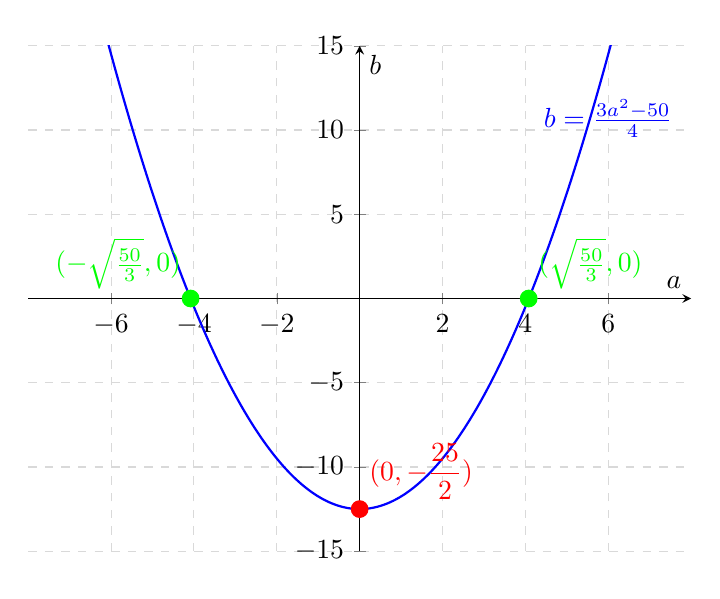
\begin{tikzpicture}
\begin{axis}[
    axis lines = center,
    xlabel = $a$,
    ylabel = $b$,
    domain = -8:8,
    samples = 100,
    grid = major,
    grid style = {dashed, gray!30},
    width = 10cm,
    height = 8cm,
    xmin = -8, xmax = 8,
    ymin = -15, ymax = 15,
    xtick = {-6, -4, -2, 0, 2, 4, 6},
    ytick = {-15, -10, -5, 0, 5, 10, 15},
]

% 関数のプロット
\addplot[blue, thick, smooth] {(3*x^2 - 50)/4};

% 頂点の点をマーク
\addplot[red, mark=*, mark size=3pt] coordinates {(0, -12.5)};

% 頂点のラベル
\node[red, above right] at (0, -12.5) {$(0, -\dfrac{25}{2})$};

% x切片をマーク
\addplot[green, mark=*, mark size=3pt] coordinates {(4.08, 0)};
\addplot[green, mark=*, mark size=3pt] coordinates {(-4.08, 0)};

% x切片のラベル
\node[green, above right] at (4.08, 0) {$(\sqrt{\frac{50}{3}}, 0)$};
\node[green, above left] at (-4.08, 0) {$(-\sqrt{\frac{50}{3}}, 0)$};

% 関数の式を表示
\node[blue, above] at (6, 9) {$b = \frac{3a^2 - 50}{4}$};

\end{axis}
\end{tikzpicture}
\\
したがって、$-5\leq a\leq 5$より、\\

$b=\dfrac{3a^2-50}{4}$の最小値は$a=-\dfrac{B}{2A}=-\dfrac{0}{2\times \dfrac{3}{4}}=0$の時、$b=-\dfrac{50}{4}=-\dfrac{25}{2}$。\\

$b=\dfrac{3a^2-50}{4}$の最大値は端点$a=\pm 5$の時、$b=\dfrac{3\times (\pm 5)^2-50}{4}=\dfrac{75-50}{4}=\dfrac{25}{4}$。\\

\noindent
従って、$b$の範囲は${\color{red}{-\dfrac{25}{2}}} \leq b \leq\color{red}{ \dfrac{25}{4}}$ となる。\\
\newpage
\section*{付録}
\hosoku\\
\noindent
\subsubsection{\textbf{\textgt{2次関数の軸と頂点の求め方}}}
二次関数 $y = ax^2 + bx + c$ を平方完成して $y = a(x - p)^2 + q$ という形にすれば,軸と頂点がわかります。具体的には,\textcolor{red}{軸は $x = p$} で\textcolor{blue}{頂点は $(p, q)$}になります。\\

\begin{tikzpicture}[scale=0.7]
    % 座標軸
    \draw[->] (-1.5, 0) -- (3, 0) node[right] {$x$};
    \draw[->] (0, -0.5) -- (0, 3) node[above] {$y$};
    \node at (-0.3, -0.3) {$O$};
    
    % 二次関数のグラフ
    \draw[thick, smooth, domain=-1:2.5] plot (\x, {0.5*(\x-1)^2 + 0.5});
    
    % 軸(対称軸)
    \draw[red, thick, dashed] (1, -0.5) -- (1, 2.5);
    \node[red] at (1, -0.6) {軸 $x = p$};
    
    % 頂点
    \fill[blue] (1, 0.5) circle (0.08);
    \fill[black] (0, 0) circle (0.08);
    \node[blue] at (2.2, 0.5) {頂点 $(p, q)$};
    
    % 関数式
    \node at (3.1, 2.1) {$y = a(x - p)^2 + q$};
\end{tikzpicture}
\\
\begin{reidai}{二次関数の軸の方程式と頂点の座標}
22次関数 $y = 2x^2 +3x - 1$ の軸の方程式と頂点の座標を求めよ。
\end{reidai}
\ \\
\kai \\

\noindent
$y = 2x^2 + 3x - 1$ を平方完成する。

\begin{align*}
y &= 2\left(x^2 + 2 \cdot \frac{3}{4}x\right) - 1\\
 &= 2\left(x + \frac{3}{4}\right)^2 - \frac{9}{8} - 1\\
 &= 2\left(x + \frac{3}{4}\right)^2 - \frac{17}{8}
\end{align*}

よって,

\begin{itemize}
\item 軸の方程式は $x = -\textcolor{red}{\frac{3}{4}}$
\item 頂点の座標は $\textcolor{blue}{\left(-\frac{3}{4}, -\frac{17}{8}\right)}$
\end{itemize}
\subsubsection{\textbf{2次関数の軸と頂点を求める公式}}
二次関数 $y = ax^2 + bx + c$ において,\\
\noindent
\textcolor{red}{軸の方程式は}\  $x = -\frac{b}{2a}$\\

\noindent
\textcolor{blue}{頂点の座標は}\  $\left(-\dfrac{b}{2a}, \dfrac{-b^2 + 4ac}{4a}\right)$
\newpage
\shomei\\


これは証明できます。まず、二次関数の一般形 $y = ax^2 + bx + c$ を考えます。平方完成を用いると、次のように変形できます。

\begin{align*}
y &= a\left(x^2 + 2\times\dfrac{b}{2a}x\right) + c \\
  &= a\left(x^2 + \dfrac{b}{2a}x\right)^2  - \left(\dfrac{b}{2a}\right)^2 + c \\
  &= a\left(x + \dfrac{b}{2a}\right)^2 + \dfrac{-b^2+4ac}{4a}
\end{align*}
\\
よって、軸の方程式は$x = -\dfrac{b}{2a}$、頂点の座標が $\left(-\dfrac{b}{2a}, \dfrac{-b^2 + 4ac}{4a}\right)$ であることがわかります。

\end{CJK}
\end{document}